\documentclass[a4,12pt]{article}

%--- Packages génériques ---%

\usepackage[english]{babel}
\usepackage[utf8]{inputenc}
\usepackage[T1]{fontenc}
\usepackage[babel=true]{csquotes}
\usepackage{amsmath}
\usepackage{amssymb}
\usepackage{textcomp}
\usepackage{float}
\usepackage{graphicx}
\usepackage{caption}
\usepackage{hyperref}
\usepackage{empheq}
\usepackage{color}
\usepackage{cancel}
\usepackage{textcomp} %% pour les intervalles d'entiers(doubles barres)

%--- Structure de la page ---%

\usepackage{fancyheadings}

\topmargin -1.5 cm
\oddsidemargin -0.5 cm
\evensidemargin -0.5 cm
\textwidth 17 cm
\setlength{\headwidth}{\textwidth}
\textheight 24 cm
\pagestyle{fancy}
\lhead[\fancyplain{}{\thepage}]{\fancyplain{}{\sl MSIAM 3A}}
\chead[\fancyplain{}{{\sl }}]{\fancyplain{}{{Summary}}}
\rhead[\fancyplain{}{}]{\fancyplain{}{Rakotonarivo \& Mazouth--Laurol}}
\lfoot{\fancyplain{}{}}
\cfoot{\fancyplain{}{}}
\cfoot{\thepage }
\rfoot{\fancyplain{}{}}

%--- Raccourcis commande ---%

\newcommand{\R}{\mathbb{R}}
\newcommand{\N}{\mathbb{N}}
\newcommand{\A}{\mathbf{A}}
\newcommand{\B}{\mathbf{B}}
\newcommand{\C}{\mathbf{C}}
\newcommand{\D}{\mathbf{D}}
\newcommand{\ub}{\mathbf{u}}

\DeclareMathOperator{\e}{e}
%--- Header to write code ---%
\usepackage { listings }
%%configuration de listings
\lstset{
	language=c++,
	basicstyle=\ttfamily\small, %
	identifierstyle=\color{black}, %
	keywordstyle=\color{blue}, %
	stringstyle=\color{black!60}, %
	commentstyle=\it\color{green!95!yellow!1}, %
	columns=flexible, %
	tabsize=2, %
	extendedchars=true, %
	showspaces=false, %
	showstringspaces=false, %
	numbers=left, %
	numberstyle=\tiny, %
	breaklines=true, %
	breakautoindent=true, %
	captionpos=b
}


\usepackage{xcolor}


\definecolor{Zgris}{rgb}{0.87,0.85,0.85}


\newsavebox{\BBbox}
\newenvironment{DDbox}[1]{
	\begin{lrbox}{\BBbox}\begin{minipage}{\linewidth}}
		{\end{minipage}\end{lrbox}\noindent\colorbox{Zgris}{\usebox{\BBbox}} \\
	[.5cm]}
%--- Mode correction et incréments automatiques ---%

\usepackage{framed}
\usepackage{ifthen}
\usepackage{comment}

\newcounter{Nbquestion}

\newcommand*\question{%
\stepcounter{Nbquestion}%
\textbf{Question \theNbquestion. }}

\newboolean{enseignant}
%\setboolean{enseignant}{true}
\setboolean{enseignant}{false}

\ifthenelse{
\boolean{enseignant}}{
\newenvironment{correction}{\begin{shaded}}{\end{shaded}}
}
{
\excludecomment{correction}
}

%%%%%%%%%%%%%%%%%%%%%%%%%%%%%%%%%%%%%%%%%%%%%%%%%%%%%%%%
% 							               EN-TETE        

\title{\textbf{Tomography reconstruction from 2D projections}}
\author{
\begin{tabular}{cc}
	\textsc{Rakotonarivo Michi} & \textsc{Maxime Mazouth--Laurol}
\end{tabular}}   
\date{\small $21^{th}$ December 2017}

\makeatletter
	\def\thetitle{\@title}
	\def\theauthor{\@author}
	\def\thedate{\@date}
\makeatother 

\usepackage{etoolbox}
\usepackage{titling}
\setlength{\droptitle}{-7em}

\setlength{\parindent}{0cm}

\makeatletter
% patch pour le bug concernant les parenthèses fermantes d'après http://tex.stackexchange.com/q/69472
\patchcmd{\lsthk@SelectCharTable}{%
  \lst@ifbreaklines\lst@Def{`)}{\lst@breakProcessOther)}\fi}{}{}{}
\begin{document}

\maketitle
\section{New results}
~~ As a reminder, for the last meeting, the sinogram has been derived for the unit disk only. Then, the idea was, using formulae relating the radon transform operator for a function $f$ and its scaled and translated variations $f_{D}$ and $f_{a}$ respectively, to derive sinograms for any disk. \\
Here are presented a few results for simple examples.
\subsection{Scaled and centered disk}
\begin{figure}[h!]
   \begin{minipage}[c]{.46\linewidth}
      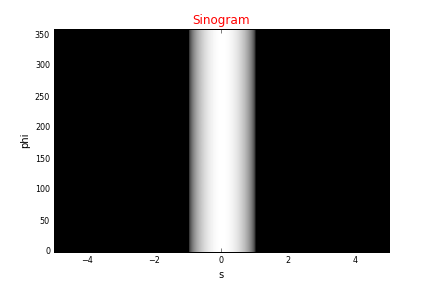
\includegraphics[scale=0.5]{../images/sinograms/unitDisk.png} 
      \captionof{figure}{Unit disk}
   \end{minipage} \hfill
   \begin{minipage}[c]{.46\linewidth}
      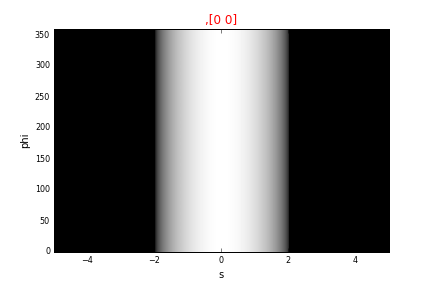
\includegraphics[scale=0.5]{../images/sinograms/scaledUnitDisk.png} 
      \captionof{figure}{Centered disk, $r=2$}
   \end{minipage}
\end{figure}
As expected, the larger is the disk, the larger the sinogram we get, proportionally to the radius.
\subsection{Translated unit disk}
\begin{figure}[h!]
   \begin{minipage}[c]{.46\linewidth}
      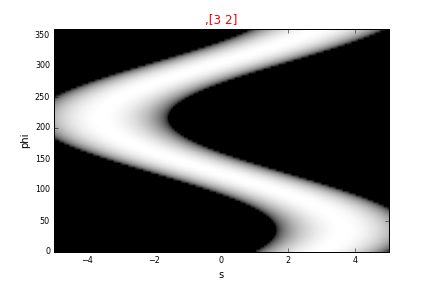
\includegraphics[scale=0.5]{../images/sinograms/translatedUnitDisk.png} 
      \captionof{figure}{translated disk, $center=(3,2)$}
   \end{minipage} \hfill
   \begin{minipage}[c]{.46\linewidth}
      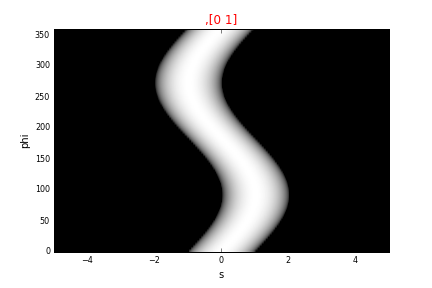
\includegraphics[scale=0.5]{../images/sinograms/translatedUnitDiskCloseCenter1.png} 
      \captionof{figure}{Centered disk, $r=2$}
   \end{minipage}
\end{figure}
For a translated disk, the sinogram has a sinusoidal shape. This can be explained by the translation formula of the previous report. \\
For any translation vector $a$, we have :
\begin{eqnarray*}
\Re f_{a}(\phi,s) &=& \Re f(\phi,s-a.\alpha_{\phi}) \\
                 &=& \Re f(\phi,s-a_{0}*\cos\phi - a_{1}*\sin\phi)
\end{eqnarray*}
Thus, the translated sinogram is the result of the composition of $\Re(B_{1})$ (radon transform on the unit disk) with a sinusoidal function with parameters $(a_0,a_1)$. It means that, the  further from the center the translated disk is, the sharper is the sinogram. 

\subsection{Translated and scaled disk}
\begin{figure}[h!]
   \begin{minipage}[c]{.46\linewidth}
      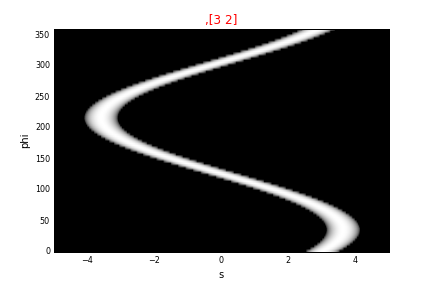
\includegraphics[scale=0.5]{../images/sinograms/translatedAndScaledDisk.png} 
      \captionof{figure}{$r=0.5$, $center=(3,2)$}
   \end{minipage} \hfill
   \begin{minipage}[c]{.46\linewidth}
      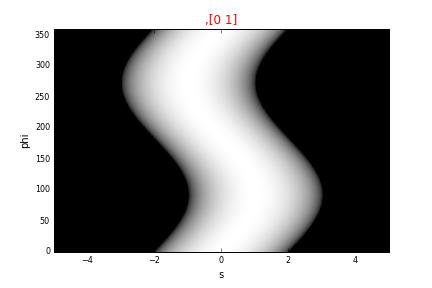
\includegraphics[scale=0.5]{../images/sinograms/translatedAndScaledDisk1.png} 
      \captionof{figure}{$r=2$, $center=(0,1)$}
   \end{minipage}
\end{figure}
Here, we can clearly see the combination of both previous properties of the radon transform operator $\Re$. \\

Then, one can obviously add several disks to the image, so that the obtained final sinogram would be the sum of each disk's sinogram.

\subsection{Fancy results}
\begin{figure}[h!]
   \begin{minipage}[c]{.46\linewidth}
      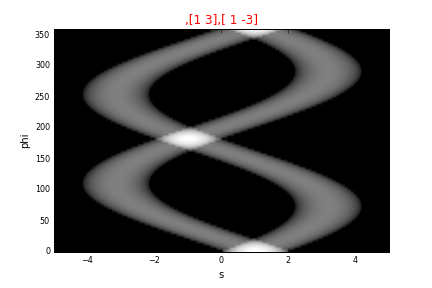
\includegraphics[scale=0.5]{../images/sinograms/2SymmetricDisks3.png} 
      \captionof{figure}{}
   \end{minipage} \hfill
   \begin{minipage}[c]{.46\linewidth}
      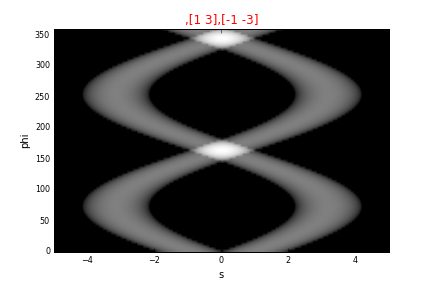
\includegraphics[scale=0.5]{../images/sinograms/2SymmetricDisks4.png} 
      \captionof{figure}{}
   \end{minipage}
\end{figure}
These are two examples of couples of symmetric disks with respect to the x-axis and the origin respectively.
\end{document}